\documentclass[runningheads]{llncs}
\usepackage[T1]{fontenc}
\usepackage[acronyms]{glossaries}
\usepackage{etoolbox}
\usepackage{xurl}
\usepackage[hidelinks]{hyperref}
\usepackage{graphicx}
\usepackage{color}
\usepackage{lipsum}
\renewcommand\UrlFont{\color{blue}\rmfamily}

\graphicspath{ {./imgs/} }

\newcommand*{\captionsource}[2]{%
  \caption[{#1}]{%
    #1%
    \\\hspace{\linewidth}%
    \textbf{Source:} #2%
  }%
}

% Redefine the glossary section style to match llncs
\makeatletter
\renewcommand{\glossarysection}[2][]{
  \section*{#2}
  \phantomsection
  \def\@glossarysection{#2}
}
\makeatother

\makenoidxglossaries{}
\loadglsentries{abbr.tex}

\begin{document}

\title{The Emergence of Deterministic Networking}
\author{Alexander Hurbean\inst{1}}
\authorrunning{Hurbean A.}
\institute{Technical University of Vienna, 1040 Vienna, Austria}

\maketitle              % typeset the header of the contribution

\begin{abstract}
  Deterministic networking is a transforming technology that changes the way real-time applications use communication networks. This paper provides a comprehensive overview of the technical foundations and enabling technologies driving deterministic networking. It also presents a historical background on how the topic of deterministic networking came to be. Key technologies are also being explored, such as \gls{tsn}, which offers features like clock synchronisation, traffic shaping, frame delay, and frame replication to make networks more reliable. Deterministic networking has applications in many different fields, such as industrial robotics, power grids, and self-driving cars. Furthermore, its compatibility with legacy networks enables a smooth transition towards deterministic behaviour. This paper shows how predictable networking could help improve communication networks for real-time applications, making them more efficient and safer. As more industries adopt deterministic networking, its transformative power is set to change how we interact and work in real-time settings, opening up new opportunities for a wide range of industries and uses.
  
  \keywords{real time, deterministic networking, time sensitive networking}
\end{abstract}

\section{Introduction}

As technology, the Internet, and industries rapidly evolve the demand for real-time applications increases and new networking challenges arise. Traditional best-effort packet delivery offered by standard Ethernet networks may not adequately meet the needs of real-time applications, such as the upcoming Industry 4.0 automation, particularly in the \gls{iot} and \gls{cps}~\cite{Wollschlaeger2017}. For instance, industrial networks began to expand beyond the confines of local area networks, necessitating deterministic characteristics across wide-area networks, such as those connecting multiple factories or linking a factory to cloud-based systems. Another issue is the various technologies currently used in industrial networks such as \gls{ecat}, and \gls{can}, which are proprietary, not interoperable, and require dedicated hardware. \gls{detnet} emerges as a key solution, providing guaranteed latency and reliability for packet data transmission even over multi-hop paths and allowing for the integration of different technologies over packet networks.

The \gls{detnet} \gls{qos} focuses on worst-case values for end-to-end latency, jitter, and packet misordering, as these values impact real-time system performance. \gls{detnet} employs three techniques, as outlined in RFC 8655~\cite{rfc8655}, to provide these \gls{qos} guarantees:

\begin{itemize}
  \item \textbf{Resource allocation}: Assigns resources such as buffer space and link bandwidth to \gls{detnet} flows, addressing latency and packet loss requirements.
  \item \textbf{Service protection}: Mitigates packet loss due to random media errors and equipment failures through mechanisms like packet replication and elimination or packet encoding. This technique distributes \gls{detnet} flows across multiple paths in time and/or space to minimize packet loss.
  \item \textbf{Explicit routes}: Provides pre-determined paths for data packets to minimize network congestion and deliver predictable performance for time-sensitive applications.
\end{itemize}

These techniques can be applied individually or in combination, with eight possible combinations, including no \gls{detnet}. Some combinations offer broader utility than others, and the \gls{detnet} architecture is designed to facilitate interoperability with existing and developing standards. Examples of typical combinations include seamless redundancy mechanisms on ring topologies, resource allocation as offered by \gls{avb}, and the use of all three techniques together for maximum protection. While simpler methods like prioritization and over-provisioning may be sufficient for some applications, \gls{detnet} provides a more comprehensive solution for critical real-time systems~\cite{rfc8655}.

This paper explores the concept of \gls{detnet}, its importance in overcoming the limitations of best-effort packet delivery, and its relevance in many real-world applications.

The paper begins with a ``Background'' section that provides a historical context and discusses the developments of \gls{detnet} and time-sensitive networking. It then examines the constraints of best-effort packet delivery and the need for specific latency and reliability guarantees for certain application classes. Additionally, an overview of proposed IEEE 802.1 standards is presented.

The paper subsequently provides an overview of different domains where \gls{detnet} plays a vital role, such as industrial automation, cellular operation, and professional multimedia. Within each domain, the use case for \gls{detnet} is being discussed, alongside the improvements that \gls{detnet} brings to the table.

Finally, the paper discusses technical foundations that enable \gls{detnet} to build on best-effort packet networks and offer the required guarantees for latency, reliability, and jitter. Key architectural components, protocols, and enabling technologies are presented, providing a general understanding of some technical foundations of \gls{detnet}.

By discussing the history, applications, and technologies underpinning \gls{detnet}, this paper aims to provide an overview and understanding of the significance of \gls{detnet}. With the continued growth of the \gls{iot}, \gls{cps}, and Industry 4.0, \gls{detnet}'s importance is poised to expand, shaping the future of connectivity.

\section{Background}

This section provides a deeper historical context of the key developments and technologies that have influenced the emergence of \gls{detnet}.

\subsection*{\gls{avb} and \gls{tsn}}
The origins of \gls{detnet} can be traced back to the development of IEEE \gls{avb} standards, which aimed to provide synchronized, low-latency streaming of audio and video data over Ethernet networks~\cite{Yang2019}. The need for such a solution stemmed from the fact that larger audio/video systems were increasingly difficult to maintain and required purpose-built hardware. Additionally, \gls{avb} allows normal Ethernet traffic to coexist with the audio/video traffic, which is a key feature for the adoption of \gls{avb} in professional environments~\cite{Lim2012}. The IEEE 802.1 task group responsible for the \gls{avb} standard renamed it to \gls{tsn} after completion to better reflect its extended scope, which includes other types of real-time traffic, such as automotive and industrial control traffic~\cite{Wollschlaeger2017}. Although \gls{avb} seemed very promising for many other applications as well, it suffered from limitations such as only supporting seven hops and only operating on Layer 2 thus not allowing communications across networks~\cite{Imtiaz2009}.

\subsection*{Industrial Fieldbus and Industrial Ethernet}
In parallel, industrial serial field bus systems, such as ProfiBus or Modbus, and industrial Ethernet, were developed to address the specific needs of automation and control systems in industrial environments since best-effort packet services, like standard Ethernet, were not suitable for such applications~\cite{Sauter2010}. The main issues with solutions such as standard Ethernet networking include high cost and unpredictability of traffic due to collisions and congestion loss~\cite{Finn2018}. Still, these early efforts laid the groundwork for the evolution of \gls{detnet}, paving the way for the advancements we see today. 

\subsection*{Wireless Solutions}
Wireless solutions have also been developed to address the need for mobility and flexibility in industrial settings. However, wireless communication has its own set of challenges, such as limited bandwidth and potential interference. To overcome these challenges, new wireless technologies such as WirelessHART~\cite{Song2008} and ISA100~\cite{Adriano2018} have been developed specifically for industrial automation and control applications. These technologies provide reliable and secure communication with low latency and high data rates, making them ideal for use in critical control systems. Despite the challenges, wireless solutions have become increasingly popular in industrial settings due to their ease of installation and flexibility.

Furthermore, the integration of 5G with \gls{tsn} and \gls{detnet} is expected to bring significant improvements to industrial communication systems. 5G's high data rates, low latency, and reliability make it a promising solution for industrial applications, while \gls{tsn} and \gls{detnet} provide deterministic guarantees for time-critical data transmission. This integration is expected to enable the development of new applications that require real-time communication and coordination between machines, such as collaborative robotics and autonomous vehicles. As such, the future of industrial communication systems looks promising, with a wide range of possibilities for increased efficiency and productivity. For example, factories could use wireless sensors to monitor equipment performance in real-time, allowing for predictive maintenance to reduce downtime and optimise production. Additionally, autonomous vehicles in a warehouse could communicate with each other and with the central control system to optimise their routes and avoid collisions, improving safety and efficiency.~\cite{Atiq2022}

\subsection*{Standardization and RFCs}
\gls{detnet} relies on various protocols and standards that are being developed and refined to cater to the needs of real-time applications. The IEEE 802.1 task group has already completed and released several \gls{tsn} standards, such as IEEE standard 802.1AS and IEEE standard 802.1CB, which play an essential role in building deterministic networks~\cite{Finn2018}.

In contrast, many standards or RFCs related to \gls{detnet} are still under development, while others have already been released. The IETF \gls{detnet} working group is responsible for creating internet-drafts for \gls{detnet}, which are works in progress and have not yet been standardized. The group is currently working on the following topics:

\begin{itemize}
  \item \gls{detnet} YANG Model
  \item \gls{detnet} Topology YANG Model
  \item \gls{detnet} Controller Plane Framework
  \item Operations, Administration and Maintenance (OAM) for \gls{detnet} with \gls{ip}/\gls{mpls} Data Plane
  \item Requirements for Scaling \gls{detnet}
\end{itemize}

Several RFCs have already been released, providing essential information about \gls{detnet} concepts and implementations:

\begin{itemize}
  \item RFC 8578: \gls{detnet} Use Cases~\cite{rfc8578}
  \item RFC 8557: \gls{detnet} Problem Statement~\cite{rfc8557}
  \item RFC 8655: \gls{detnet} Architecture~\cite{rfc8655}
  \item RFC 8939: \gls{detnet} Data Plane: IP~\cite{rfc8939}
  \item RFC 8964: \gls{detnet} Data Plane: MPLS~\cite{rfc8964}
  \item RFC 9023: \gls{detnet} Data Plane: IP over IEEE 802.1 TSN~\cite{rfc9023}
\end{itemize}

Standards concerning \gls{tsn} are already finished and released by the IEEE 802.1 task group, such as IEEE standard 802.1AS or IEEE standard 802.1CB which can be used to aid in building deterministic networks~\cite{Finn2018}.

\section{Overcoming the Limitations of Best-Effort Packet Delivery}

The limitations of the Internet's best-effort packet delivery service have been a challenge for applications that require specific latency and reliability guarantees. For instance, industrial control systems, telemedicine, and financial trading require timely and predictable packet delivery. The traditional approach of overprovisioning the network to ensure performance is not scalable and can be prohibitively expensive. Therefore, there is a need for a new networking paradigm that provides deterministic guarantees for specific traffic flows. This is where \gls{detnet} comes in. \gls{detnet} is an architecture that enables deterministic packet forwarding and delivery in a network~\cite{Finn2018}. An example of how this architecture can look can be seen in Figure~\ref{fig:detnet-architecture}. The subnetworks shown in Figure~\ref{fig:detnet-architecture} can be implemented using \gls{tsn}, \gls{mpls} or optical transport network~\cite{rfc8655}. For more information on this refer to the \gls{detnet} architecture RFC~\cite{rfc8655}.

\begin{figure}[ht]
  \centering
  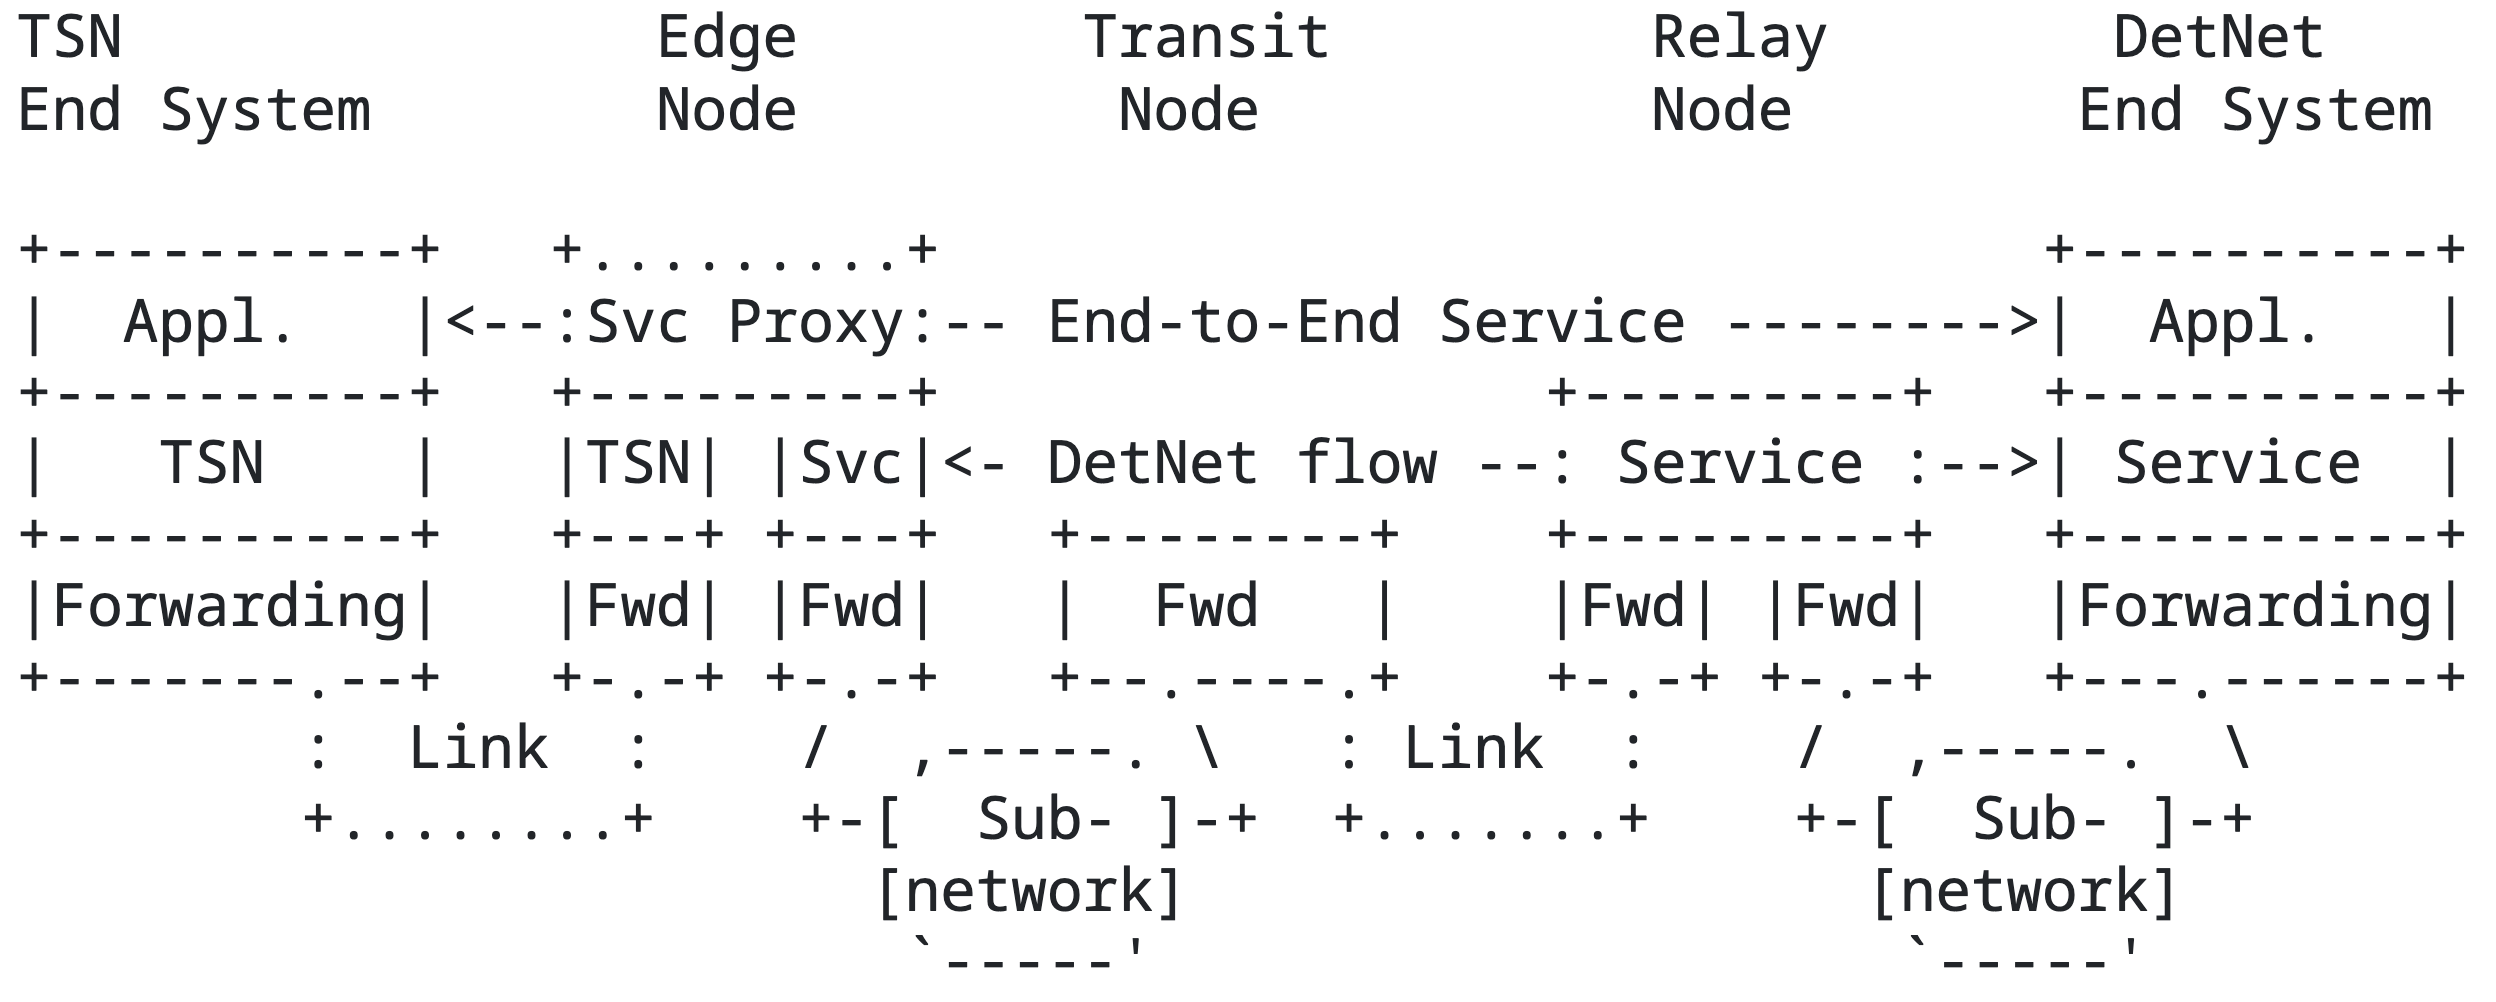
\includegraphics[width=0.7\textwidth]{detnet_simple_arch}
  \captionsource{Example of a \gls{detnet} architecture}{\url{https://www.comsoc.org/publications/ctn/quick-and-dead-rise-deterministic-networks} \& RFC8655\cite{rfc8655}}
  \label{fig:detnet-architecture}
\end{figure}

An example of \gls{detnet} in action can be seen in a factory that relies on real-time control systems. With \gls{detnet}, critical control packets can be given priority and delivered with low jitter and high reliability, ensuring that the machines on the factory floor are properly automated and operate efficiently. This also allows for better coordination between different machines and processes, making the entire system more responsive and reliable overall~\cite{rfc8578}.

\gls{detnet} achieves this by reserving network resources, such as bandwidth and buffer space for specific traffic flows and providing strict latency and reliability guarantees. \gls{detnet} also supports traffic engineering and congestion control to ensure that network resources are used efficiently. \gls{detnet} is particularly useful for applications that require real-time communication, such as industrial automation and multimedia streaming. In addition, \gls{detnet} can also improve the performance of traditional best-effort applications by providing more predictable network behavior, by being an extension to Ethernet and allowing currently existing networks to be extended and built upon~\cite{rfc8578}.

To overcome the limitations of best-effort packet delivery, \gls{detnet} leverages various technologies and techniques. Some of these include:

\begin{itemize}
  \item \gls{tsn}: \gls{tsn} is a set of IEEE 802.1 standards that provide deterministic guarantees for Ethernet-based networks, which can be applied in \gls{detnet} environments~\cite{rfc9023}.
  \item Path redundancy: \gls{detnet} employs frame replication and elimination mechanisms to ensure that critical messages have multiple paths to their destination, increasing reliability and fault tolerance~\cite{rfc8655}. In addition to that, a packet ordering mechanism is used to ensure that packets are reordered in the correct order, which may be needed for time-sensitive applications~\cite{ietf-detnet-pof-02}.
  \item Network slicing: This approach allows network operators to dedicate specific resources and create virtual networks with deterministic guarantees for specific applications~\cite{Bhattacharjee2021,rfc8578}.
\end{itemize}

However, implementing \gls{detnet} requires changes to the network infrastructure and protocols, which can be challenging and time-consuming. One of the key challenges of implementing \gls{detnet} is ensuring interoperability with existing network protocols and equipment. \gls{detnet} requires brand-new protocols and mechanisms for resource reservation, traffic engineering, and congestion control that legacy network devices might not be able to support. Therefore, network operators may need to upgrade their equipment or deploy new hardware that supports \gls{detnet}. In addition, \gls{detnet} may also require changes to the network architecture, such as the deployment of edge computing and network slicing, to provide end-to-end determinism~\cite{rfc8655}.

Despite these challenges, \gls{detnet} has the potential to revolutionize the way we design and operate networks, providing unprecedented levels of reliability and predictability for critical applications. As such, it is an area of active research and development, with ongoing efforts to standardize and commercialize \gls{detnet} technologies. While the road ahead may be challenging, the benefits of \gls{detnet} are clear, and it is likely to play an increasingly important role in the future of networking.

\section{Real-World Applications of Deterministic Networking}

Deterministic networking has numerous real-world applications across various domains, offering significant benefits in terms of reliability, predictability, and efficiency. All examples have been taken from the \gls{detnet} use cases document~\cite{rfc8578}.

\subsection{Professional Audio and Video}
Deterministic networking is essential for professional audio and video applications, where high-quality and reliable transmission of streams is vital. Key use cases include uninterrupted and synchronized stream playback, sound reinforcement, and secure transmission. The technology enables the integration of Layer 3 interconnecting Layer 2 islands, ensuring high-reliability stream paths and seamless integration of reserved streams into IT networks.

Furthermore, deterministic networking supports traffic segregation, latency optimization by a central controller, and reduced device costs due to reduced buffer memory. By utilizing packet-forwarding rules, VLANs, and subnets, deterministic networking ensures that critical audio and video streams are transmitted securely and efficiently over networks.

\subsection{Electrical Utilities}
Electrical utilities can greatly benefit from deterministic networking in several use cases. For transmission, deterministic networking is applied in protection, intra-substation process bus communications, and wide-area monitoring and control systems. In generation use cases, it plays a role in controlling the generated power and generation infrastructure management. In distribution use cases, deterministic networking helps in \gls{flisr}.

By adopting deterministic networking, electrical utilities can migrate to packet-switched networks and meet the growing telecommunications and security requirements. This migration ensures that utilities can efficiently manage their networks while enhancing security and reliability.

\subsection{\gls{bas}}
Building automation systems can leverage deterministic networking for various applications such as environmental monitoring, fire detection, and feedback control. With deterministic networking, \gls{bas} architecture can be designed to guarantee end-to-end delivery of data and support the integration of standardized data-flow information models.

Deterministic networking ensures that building automation systems can maintain a high level of efficiency, safety, and responsiveness in diverse environments, paving the way for smarter and more sustainable buildings.

\subsection{Wireless for Industrial Applications}
Deterministic networking is crucial for wireless industrial applications, where network convergence using 6TiSCH\footnote{6TiSCH (IPv6 over the TSCH mode of IEEE 802.15.4e) is a networking protocol that combines IPv6 and the Time-Slotted Channel Hopping (TSCH) mode of IEEE 802.15.4e standard. It provides deterministic communication capabilities in low-power and lossy networks by dividing time into fixed-length timeslots and allocating them for scheduled transmission of data~\cite{Vilajosana2020,Dujovne2014}.} and common protocol development is essential~\cite{rfc9023}. By employing deterministic networking, unified wireless networks and management can be achieved, increasing reliability and scalability in industrial settings.

In this context, deterministic networking allows for efficient schedule management by a \gls{pce} and facilitates 6TiSCH security considerations, ensuring a robust and secure wireless network for industrial applications.

\subsection{Cellular Radio}
In cellular radio networks, deterministic networking addresses key challenges such as delay constraints, time-synchronization constraints, and transport-loss constraints. By ensuring network security, deterministic networking can enhance fronthaul, midhaul, and backhaul networks in future cellular radio systems, leading to improved performance and reliability.

\subsection{Industrial \gls{m2m}}
In industrial \gls{m2m} communications, deterministic networking ensures reliable and predictable communication between machines, sensors, and control systems. It has the potential to replace multiple proprietary deterministic networks, lowering the overall cost of multi-vendor solutions and providing a more unified and standardized communication platform for industrial applications.

\subsection{Mining Industry}
In the mining industry, deterministic networking can offer reliable and secure communication between machines, sensors, and control systems, allowing for increased safety and efficiency in mining operations. By ensuring predictable and reliable data transmission, deterministic networking can help prevent accidents and improve the overall productivity of mining processes.

\subsection{Private Blockchain}
Private blockchain networks can benefit from deterministic networking, which ensures reliable and secure communication between nodes and facilitates efficient blockchain operations. By guaranteeing deterministic communication, private blockchain networks can maintain high levels of security and performance, enabling the secure and efficient exchange of information and transactions.

\subsection{Network Slicing}
In network slicing, deterministic networking plays a crucial role in providing end-to-end service assurance and managing multiple virtual networks on a shared infrastructure. Network slicing allows operators to customize different network slices for various use cases, such as industrial automation, \gls{iot}, and critical communication services, ensuring each slice has the required performance and reliability.

Deterministic networking ensures that each slice maintains its \gls{qos} requirements by guaranteeing deterministic data transfer and resource allocation. This enables service providers to offer tailored solutions to customers, ensuring the efficient use of network resources and the delivery of high-quality services.

\subsection{Automotive Industry (IEE P802.1DG)}
The automotive industry can greatly benefit from deterministic networking in various applications such as \gls{adas}, autonomous driving, and \gls{v2x} communication. Deterministic networking ensures reliable and predictable communication between vehicles, sensors, and control systems, enabling real-time decision-making and enhanced safety on the roads.

In autonomous driving, deterministic networking provides low-latency communication, ensuring that vehicles can share critical information and make accurate decisions in a timely manner. Additionally, deterministic networking can support \gls{v2x} communication, enabling seamless communication between vehicles, infrastructure, and pedestrians for improved traffic management and safety.

\subsection{Aerospace and Defense (IEEE P802.1DP / SAE AS6675)}
In the aerospace and defense industry, deterministic networking plays a vital role in applications such as air traffic control systems, satellite communication, and military communication networks. These systems require reliable, secure, and predictable communication to ensure the safety of air travel and the success of defense missions.

Deterministic networking ensures that critical data is transmitted with minimal latency and maximum reliability in these high-stakes environments, contributing to the overall safety and efficiency of aerospace and defense operations.

\subsection{Healthcare}
In the healthcare industry, deterministic networking is essential for applications such as telemedicine, remote surgery, and patient monitoring. These applications require reliable and predictable communication to ensure patient safety and the success of medical procedures~\cite{Zhang2022}.

Deterministic networking guarantees the timely transmission of critical data, such as real-time video feeds and sensor data, enabling healthcare professionals to make accurate decisions and perform procedures with the utmost precision. This technology contributes to the advancement of healthcare services and improved patient outcomes.

In conclusion, deterministic networking is a critical technology that has the potential to revolutionize numerous industries by ensuring reliable, secure, and predictable communication. Its applications span across various domains, including professional audio and video, electrical utilities, building automation systems, wireless industrial applications, cellular radio, industrial \gls{m2m}, mining, private blockchain, network slicing, automotive, aerospace and defense, and healthcare. By adopting deterministic networking, these industries can reap the benefits of improved efficiency, safety, and performance, paving the way for a more connected and reliable future.

\section{The Technical Foundations of Deterministic Networking}
One of the key enabling technologies for deterministic networking is \gls{tsn}, which is a set of IEEE 802.1 standards that provide deterministic guarantees for Ethernet-based networks. \gls{tsn} offers a range of features, such as time synchronization, traffic shaping, and path redundancy, that enable deterministic behavior in the network. By using \gls{tsn}, deterministic networking can provide low-latency, high-reliability communication for a variety of applications. Another important aspect of deterministic networking is its ability to coexist with legacy networks, allowing for a gradual migration towards deterministic behavior.

\subsection*{Clock Synchronization}
One of the fundamental requirements for deterministic networking is clock synchronization. In a time-triggered network, all devices must have a common notion of time to ensure that data is transmitted at the correct time. This requires accurate clock synchronization across the network, which can be achieved using protocols such as \gls{ptp} or \gls{tsn}. \gls{ptp} is a widely adopted standard for clock synchronization in industrial automation and power grids, while \gls{ptp} offers enhanced clock synchronization capabilities for Ethernet-based networks. By ensuring accurate clock synchronization, deterministic networking can provide reliable and predictable communication for real-time applications.

\subsection*{Time Aware Shaper (IEEE 802.1Qbv)}
Another key technology for deterministic networking is the \gls{tas}, which is a traffic shaping mechanism that ensures that data is transmitted at the correct time. In a time-triggered network, data must be transmitted in fixed time slots to ensure that it arrives at its destination on time. \gls{tas} enforces this requirement by shaping traffic according to a predefined schedule, which is determined by the network topology and traffic patterns. As Figure~\ref{fig:tas} shows, the \gls{tas} opens and closes queues with differently classed traffic based on time and the gate control list. By using \gls{tas}, deterministic networking can provide low-latency, high-reliability communication for a variety of applications.

\begin{figure}[ht]
  \centering
  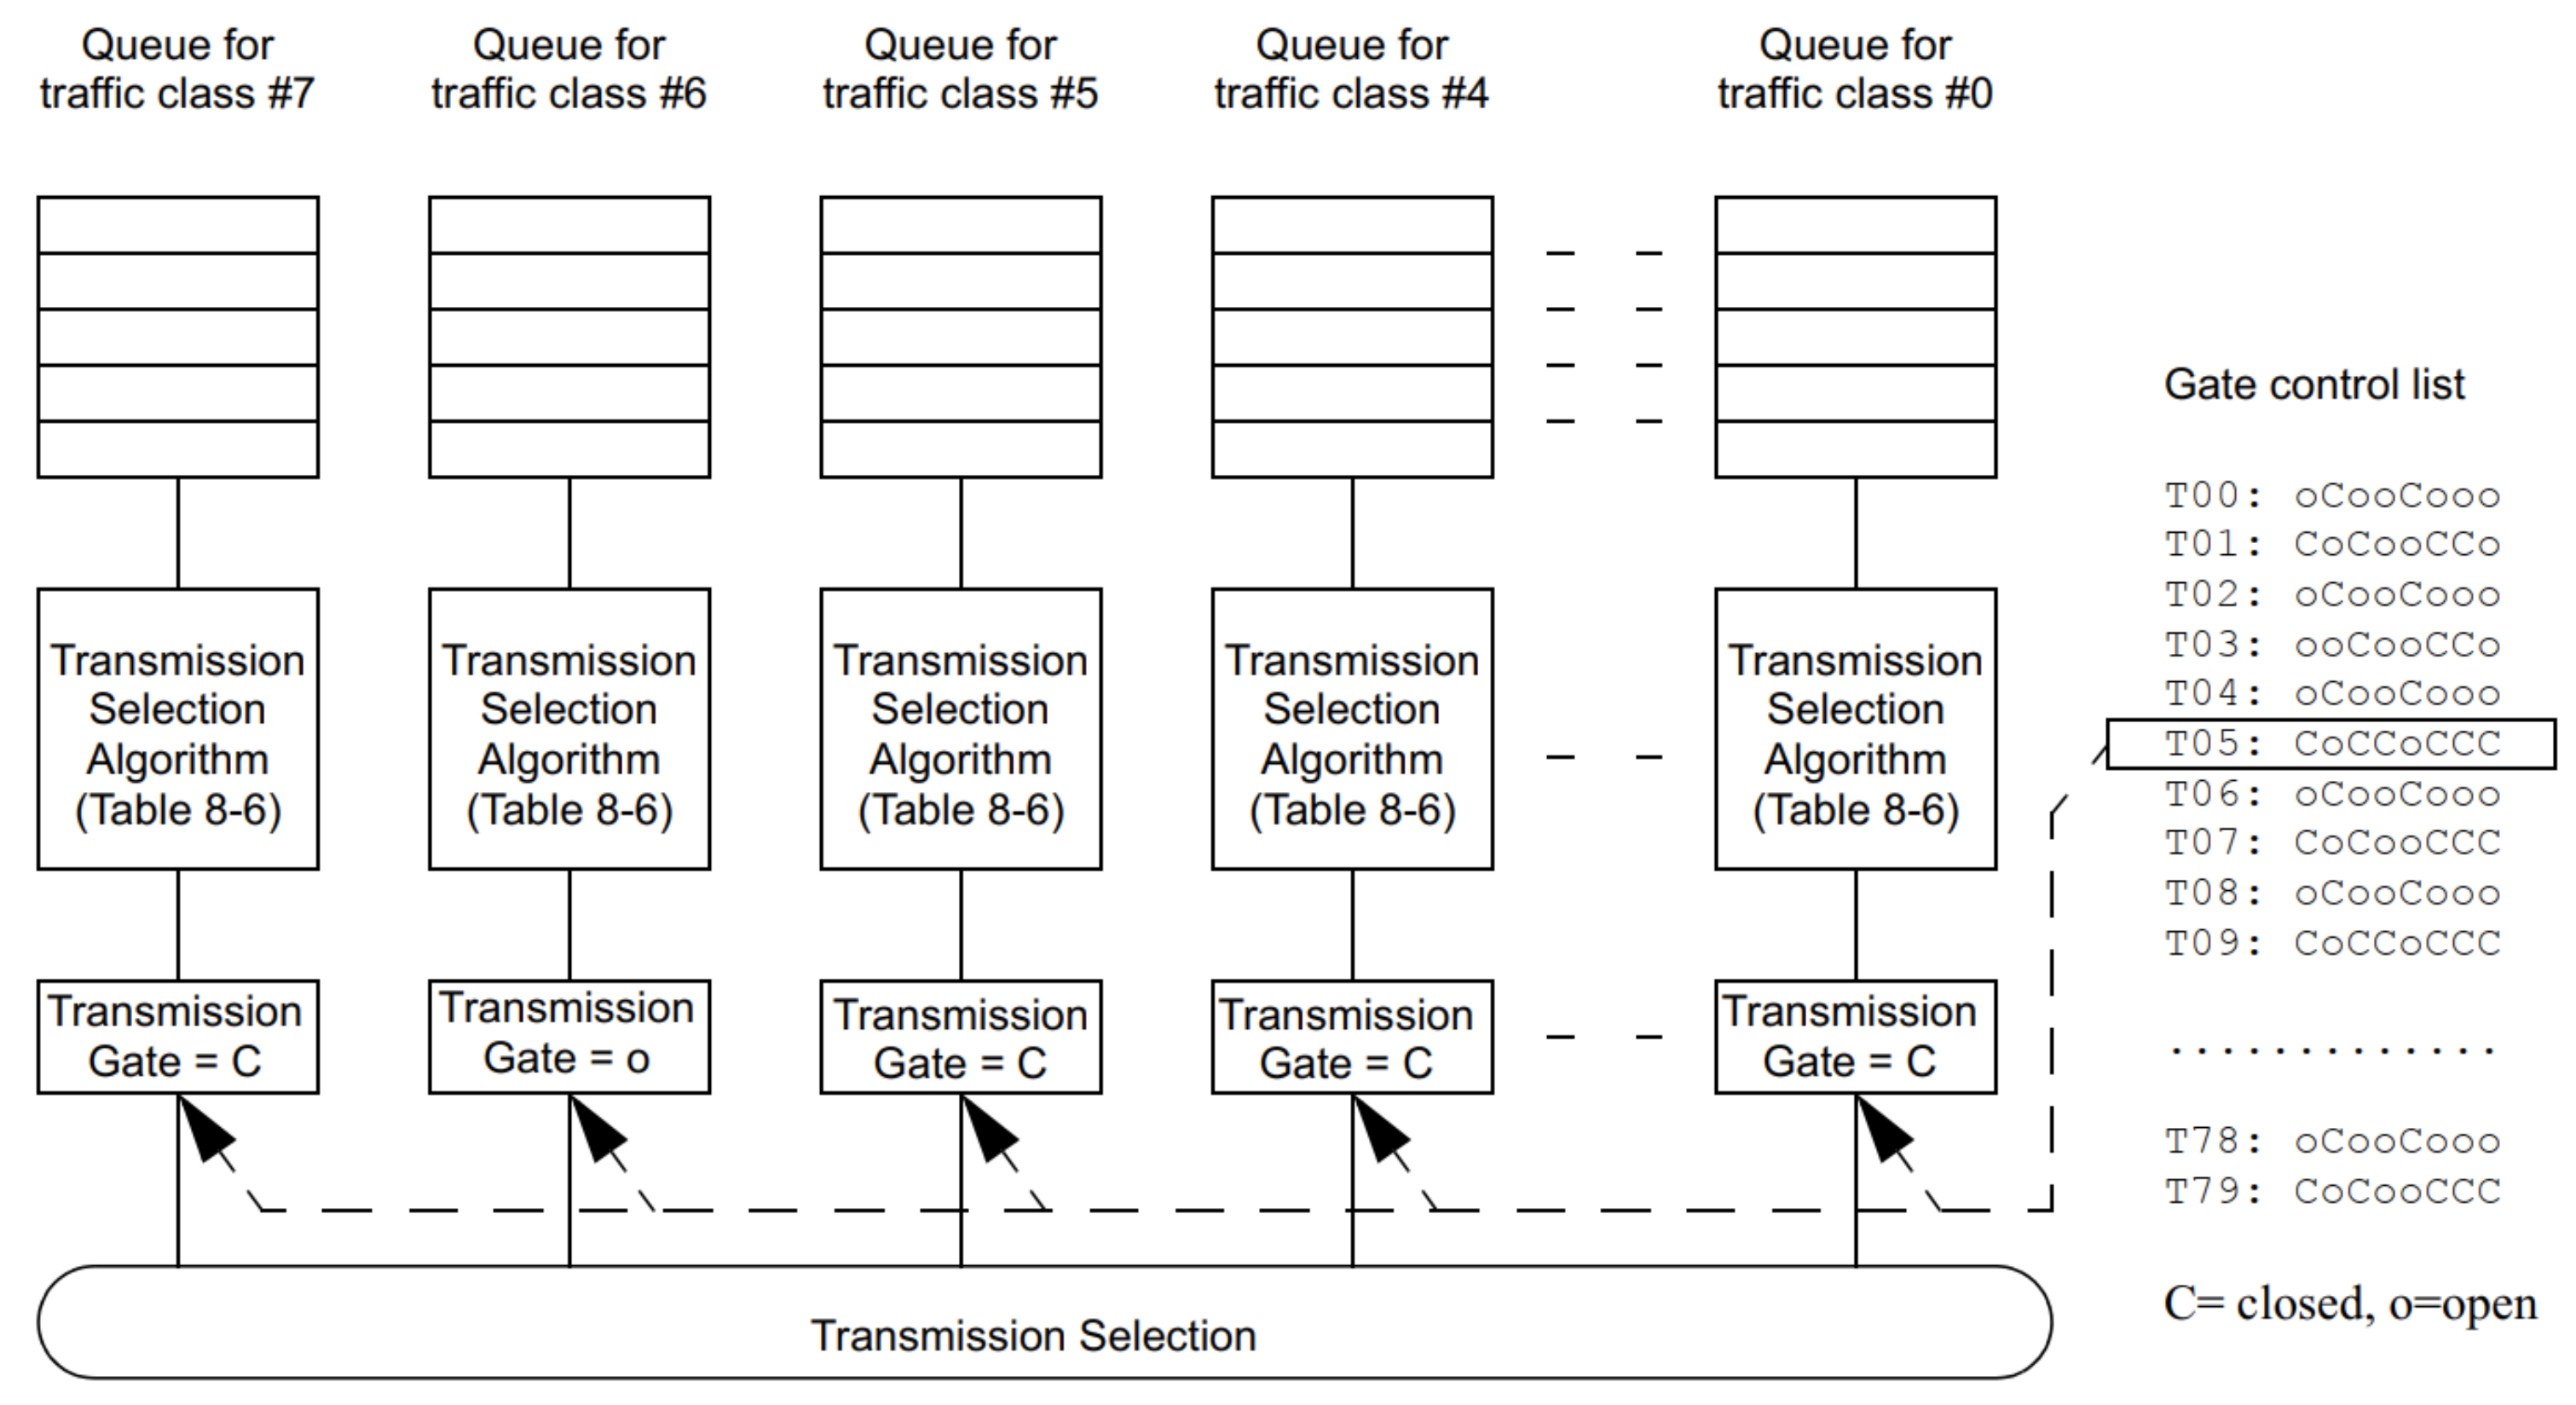
\includegraphics[width=0.8\linewidth]{tas}
  \captionsource{Time Aware Shaper Diagram}{Kellermeier et al.~\cite{Kellermeier2018}}
  \label{fig:tas}
\end{figure}

\subsection*{Frame Preemption (IEEE 802.1Qbu)}
Another important \gls{tsn} feature is frame preemption, which allows high-priority traffic to interrupt and preempt lower-priority traffic in real-time. This ensures that critical messages are delivered without delay, even in congested network conditions. Frame Preemption works by inserting a special message, called a preemption frame, into the network that signals the lower-priority traffic to pause transmission and allows the high-priority traffic to be transmitted immediately. Figure~\ref{fig:fpem} shows how frame preemption allows time-critical traffic to be transmitted immediately, thus lowering its perceived latency. This feature is particularly useful in industrial automation and control systems, where real-time communication is essential for safety and efficiency.

\begin{figure}[ht]
  \centering
  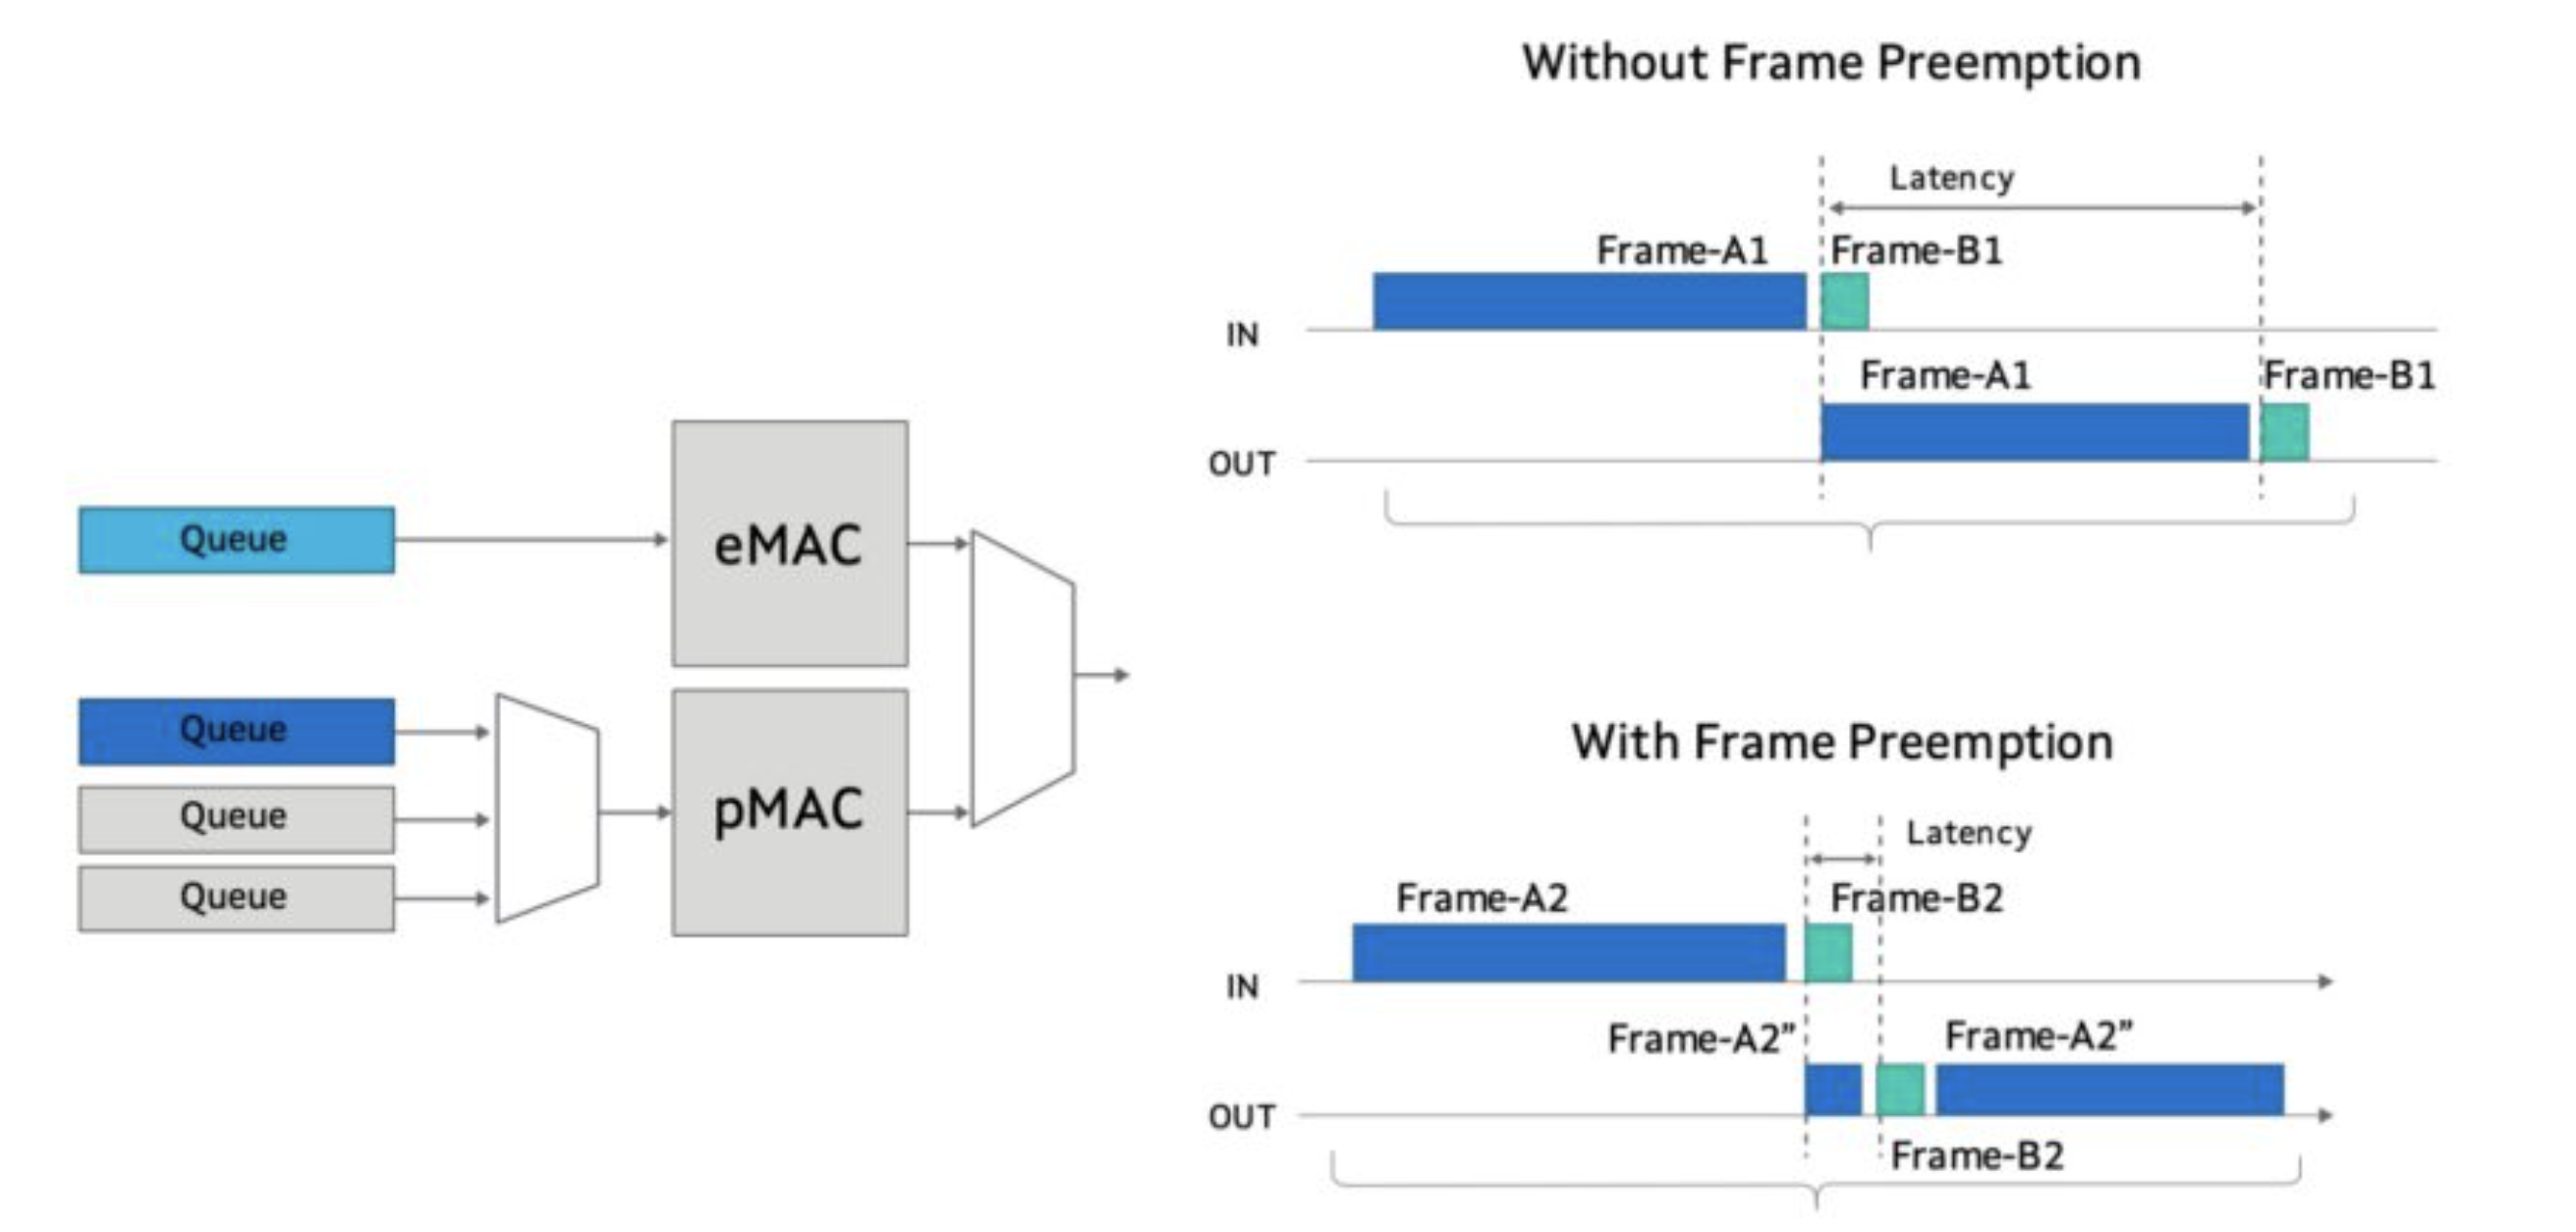
\includegraphics[width=\linewidth]{frame_preemption}
  \captionsource{Frame Preemption Diagram}{\url{https://cn.marvell.com/blogs/2022/11/tsn-and-prestera-dx1500-a-bridge-across-the-it-ot-divide/}}
  \label{fig:fpem}
\end{figure}

\subsection*{Frame Replication and Elimination for Reliability (IEEE 802.1CB)}
\gls{frer} is a \gls{tsn} feature that provides redundancy for critical traffic (see Figure~\ref{fig:frer}). It works by replicating critical messages and sending them over multiple paths to ensure that at least one copy reaches its destination. If a message is lost or corrupted on one path, it can be recovered from another path. This feature is particularly useful in industrial automation and control systems, where reliability is essential for safety and efficiency.

\begin{figure}[ht]
  \centering
  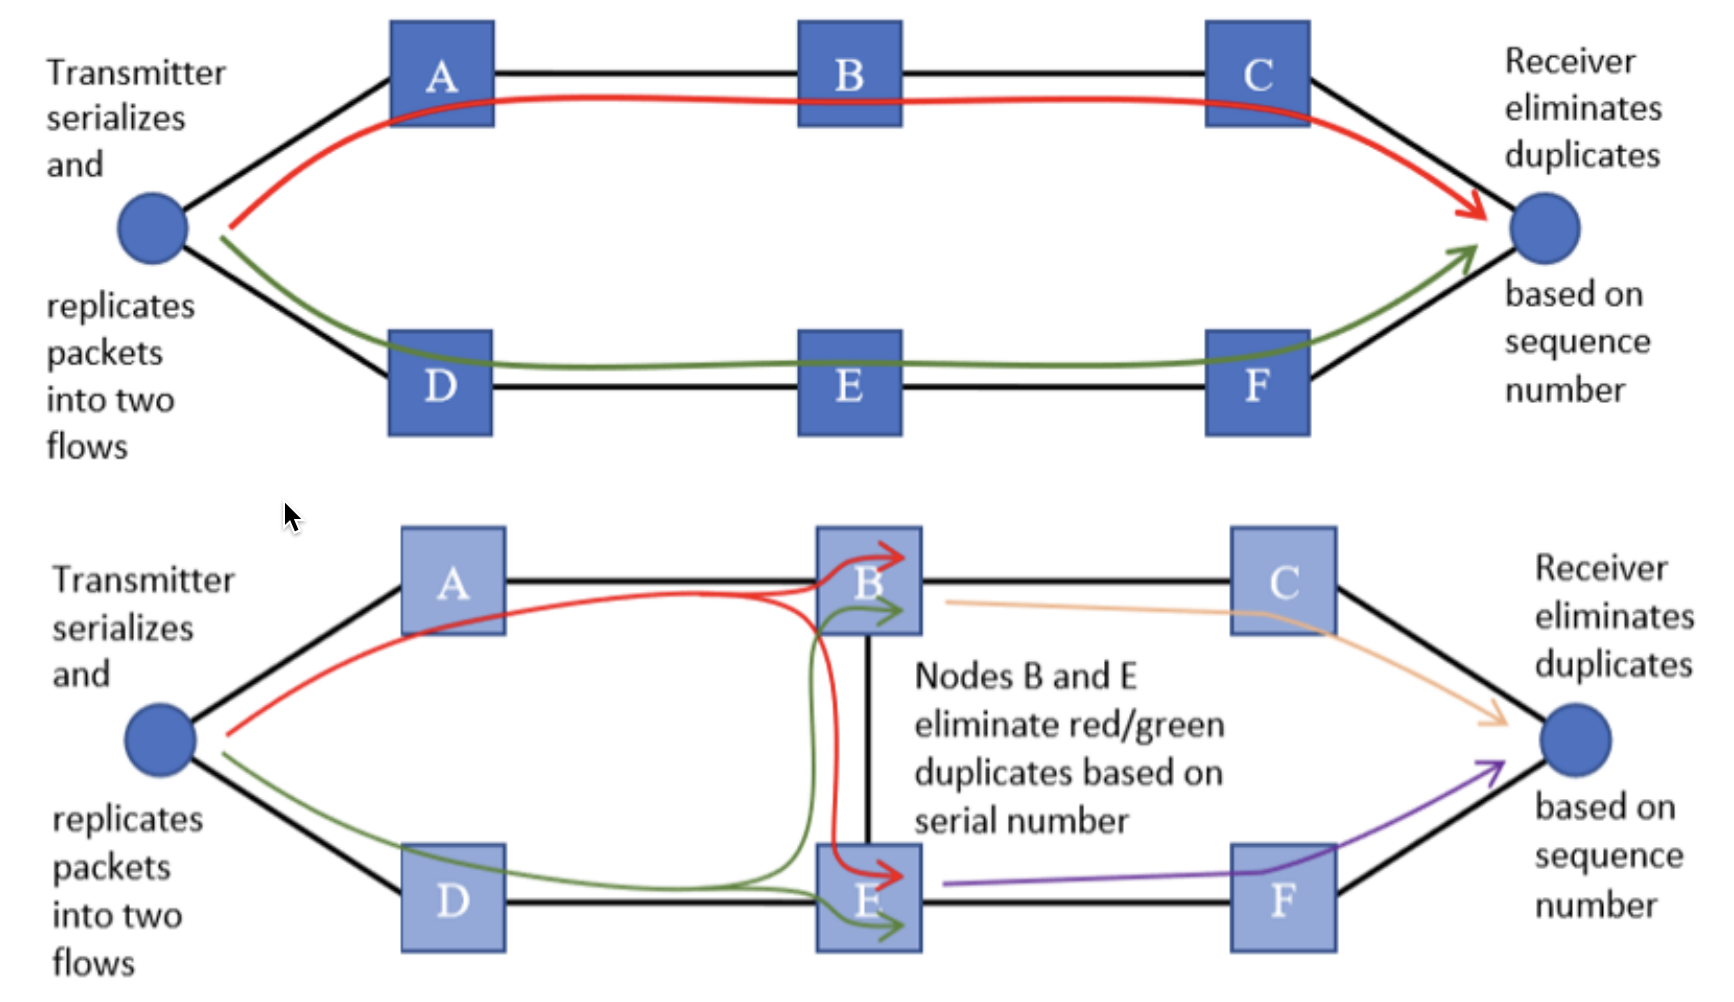
\includegraphics[width=0.8\linewidth]{frer}
  \captionsource{Mechanisms of frame replication and elimination}{Yang et al.~\cite{Yang2019}}
  \label{fig:frer}
\end{figure}

\subsection*{Network Slicing}
Network slicing is another critical aspect of deterministic networking, enabling the partitioning of network resources to support different types of traffic with varying requirements. By creating virtual network slices, each with their own \gls{qos} guarantees, deterministic networking can ensure that real-time applications receive the necessary resources and performance guarantees while coexisting with non-real-time traffic~\cite{ietf-teas-ietf-network-slices-19}.

In addition to \gls{tsn}, network slicing can be achieved using technologies such as \gls{sdn} and \gls{nfv}. These technologies enable the dynamic allocation of network resources to meet the requirements of different applications, providing an additional layer of flexibility and adaptability in deterministic networks.

In summary, deterministic networking leverages a variety of technologies, such as \gls{tsn}, clock synchronization, traffic shaping, frame preemption, and network slicing, to provide predictable and reliable communication networks for real-time applications. These technical foundations enable deterministic networking to support critical use cases in industrial automation, power grids, autonomous vehicles, and other sectors, providing a robust and efficient communication infrastructure for the future.

\section{Conclusion}

In conclusion, deterministic networking is a game-changing technology that delivers predictable and reliable communication networks, crucial for real-time applications. Built on a time-triggered architecture, deterministic networking employs protocols that prioritize traffic, guarantee timely delivery, and minimize packet loss. \gls{tsn} serves as a pivotal enabling technology, providing deterministic assurances for Ethernet-based networks.

The potential of deterministic networking to transform industries and applications such as industrial automation, power grids, and autonomous vehicles is immense. Its compatibility with existing legacy networks enables a smooth transition towards deterministic behavior, facilitating widespread adoption across various sectors.

Ultimately, deterministic networking has the potential to revolutionize the way we communicate and interact with real-time applications, leading to greater efficiency, safety, and performance. As more industries recognize its benefits and integrate deterministic networking into their operations, its impact will only continue to grow, shaping the future of communication networks.

\printnoidxglossary[type=acronym,sort=letter,title=Abbreviations]

\bibliographystyle{splncs04}
\bibliography{export}
\end{document}
